% !TeX root = ../correctness-deciders.tex

\section{Bouncers}\label{sec:bouncers}

\paragraph{Acknowledgement.}  Sincere thanks to Tony Guilfoyle who initially implemented a decider for bouncers\footnote{See: \url{https://github.com/TonyGuil/bbchallenge/tree/main/Bouncers}.}.
Others have contributed to this method by producing alternative implementations (see Section~\ref{sec:bouncers-implem}) or discussing and writing the formal proof presented here: savask, Iijil, mei, Tristan Stérin (cosmo).


\begin{figure}[h!]
    \centering
    \includegraphics*[width=0.9\textwidth]{figures/bouncers/bouncers.pdf}
    \caption{Space-time diagrams (10,000 steps) of several \texttt{bbchallenge} \textit{bouncers}: (a) simple bouncer bouncing back and forth between expanding tape extremeties while writing 1s (b) bouncer with more complex alternating \textit{repeater} patterns left and right of the origin (c) unilateral bouncer with a complex \textit{wall} pattern at the origin (d) unilateral bouncer, main example used throughout this section (e) bouncer entering a repetitive bouncing pattern after $\sim$6,000 steps (bottom half of the image).}\label{fig:bouncers}
\end{figure}

\subsection{Characterising bouncers}

Intuitively, a \emph{bouncer} is a Turing machine that populates a tape with
linearly-expanding patterns, called \textit{repeaters}, possibly separated or enclosed by fixed patterns called \textit{walls}. This intuitive definition corresponds to a wide range of behaviors, from simply bouncing back and forth between the tape's expanding extremities, Figure~\ref{fig:bouncers}~(a), to complex traversal of \textit{repeater} and \textit{wall} patterns, Figure~\ref{fig:bouncers}~(b)-(d), and possibly a delayed onset of the \textit{bouncing} pattern, Figure~\ref{fig:bouncers}~(e). What we call bouncers is a generalisation of the various classes of ``Christmas trees'' used to solve $\text{BB}(4)$ \cite{Brady83}.

The goal of this section is to formally characterise bouncers and show that they do not halt, see Theorem~\ref{th:bouncers}. Then, in Section~\ref{sec:bouncers-implem}, we show how do detect bouncers algorithmically in practice, see Algorithm~\ref{alg:decider-bouncers}.

\subsubsection{Directional Turing machines}\label{sec:bouncers:directionalTM}

We build on the concept of directional Turing machine introduced in Section~\ref{sec:conventions}. Directional Turing machines are an equivalent formulation of Turing machines where the machine head lives in between the tape cells and can point to the left or to the right. We choose here to treat $0^\infty$ as a unique symbol (instead of an infinite collection of 0s) and write $\overline{\Sigma} = \{0^\infty\}\cup\Sigma$, with $\Sigma$ the tape alphabet of the machine -- in the context of $\text{BB}(5)$, we have $\Sigma=\{0,1\}$. For each Turing machine with set of states $S$ we introduce 2$|S|$ new configuration symbols (i.e.\ symbols used to describe machine configurations and not read/write symbols) denoting the machine head in two possible orientations, namely $\Delta = \{\lhead s | s\in S\}\cup\{\rhead s| s \in S\}$.

We define a \textit{tape}\footnote{Note that in the terminology of Section~\ref{sec:conventions}, the definition of a tape that we use here, where the head in part of the tape, corresponds to a (partial) TM configuration.} to be a finite word of the form $uhv$, where $u,v\in \overline{\Sigma}^*$ and $h\in\Delta$, moreover, $u$ and $v$ must have at most one occurrence of $0^\infty$ each, respectively as first symbol for $u$ or last symbol for $v$. We choose the initial tape to be $0^\infty \rhead{\text{A}} 0^\infty$. Now, we define tape rewrite rules which will be used to simulate a directional Turing machine which we fix from now on. Suppose that for $s\in S, x\in \Sigma$ we have $\delta(s,x) = (s',d,x')$ where $s'\in S, d \in \{\text{L},\text{R}\}, x' \in \Sigma$ and $\delta$ the transition function of the machine, then we define the following tape rewrite rules:


\begin{table}[h!]
    \centering
    \begin{tabular}{l|l}
        If $d = \text{L}$                               & If $d = \text{R}$ \\
        \hline
        $\begin{aligned}[t]
                 x \lhead{s}\,\,\, & \to \,\,\, \lhead{s'} x' \\
                 \rhead{s} x\,\,\, & \to \,\,\, \lhead{s'} x'
             \end{aligned}$ & $\begin{aligned}[t]
                                   x \lhead{s}\,\,\, & \to \,\,\, x' \rhead{s'} \\
                                   \rhead{s} x\,\,\, & \to \,\,\, x' \rhead{s'}
                               \end{aligned}$     \\
        \hline
    \end{tabular}\\
    \ \\ If $x=0$, also define: \\
    \begin{tabular}{l|l}
        \hline
        $\begin{aligned}[t]
                 0^\infty \lhead{s}\,\,\, & \to \,\,\, 0^\infty \lhead{s'} x'   \\
                 \rhead{s} 0^\infty\,\,\, & \to \,\,\, \lhead{s'} x'\, 0^\infty
             \end{aligned}$ & $\begin{aligned}[t]
                                   0^\infty \lhead{s}\,\,\, & \to \,\,\, 0^\infty \, x' \rhead{s'} \\
                                   \rhead{s} 0^\infty\,\,\, & \to \,\,\, x' \rhead{s'} 0^\infty
                               \end{aligned}$ \\
        \hline
    \end{tabular}\\
\end{table}

Given a tape $t=uvw$ and a word $t'=uv'w$, with $u,w\in \overline{\Sigma}^*$, $v,v' \in ( \overline \Sigma \cup \Delta)^*$, suppose that there is a rewrite rule $v \to v'$. Then $t'$ is also a tape and in this situation we write $t \vdash t'$ meaning that $t'$ is obtained from $t$ by one simulation step; note that the definition is sound because, to any given tape, at most one rewrite rule applies, hence $v \to v'$ is defined uniquely and so is $t \vdash t'$. Note that the only case where $\vdash$ is not defined on a tape is if the machine halts in this configuration, i.e.\ an undefined transition is reached. Applying $\vdash$ successively $n\in\mathbb{N}$ times is written $\vdash^n$. The transitive closure of $\vdash$ (i.e.\ applying $\vdash$ \textit{some} nonzero number of times) is written $\vdash^*$.

\begin{example}\label{ex:bouncer88427177}
    Consider \texttt{bbchallenge} machine\footnote{Accessible at \url{https://bbchallenge.org/88427177}} \#88,427,177 (Figure~\ref{fig:bouncers}~(d)), that has the following transition table:
    \[
        \begin{array}{l|ll}
              & 0          & 1          \\
            \hline
            A & 1\text{RB} & 1\text{LE} \\
            B & 1\text{LC} & 1\text{RD} \\
            C & 1\text{LB} & 1\text{RC} \\
            D & 1\text{LA} & 0\text{RD} \\
            E & \mbox{---} & 0LA
        \end{array}
    \]

    Given the above definitions, we will have the following rewrite rules with state A on the left-hand side:
    \begin{align*}
        0 \lhead{A}\,\,\,        & \to\,\,\, 1 \rhead{B}          \\
        \rhead{A} 0\,\,\,        & \to\,\,\, 1 \rhead{B}          \\
        1 \lhead{A}\,\,\,        & \to\,\,\, \lhead{E} 1          \\
        \rhead{A} 1\,\,\,        & \to\,\,\, \lhead{E} 1          \\
        0^\infty \lhead{A}\,\,\, & \to\,\,\, 0^\infty 1 \rhead{B} \\
        \rhead{A} 0^\infty\,\,\, & \to\,\,\, 1 \rhead{B} 0^\infty
    \end{align*}
    The other rewrite rules are those with left-hand side states B, C, D and E. Simulating the machine for 4 steps, starting from initial tape yields:
    $ 0^\infty \rhead{\text{A}} 0^\infty \;\vdash\; 0^\infty \, 1 \rhead{\text{B}} 0^\infty \;\vdash\; 0^\infty \, 1 \lhead{\text{C}} 1\, 0^\infty\ \;\vdash\; 0^\infty \, 1 \rhead{\text{C}} 1\, 0^\infty \;\vdash\; 0^\infty \, 1 1 \rhead{\text{C}} 0^\infty$. Hence, $0^\infty \rhead{\text{A}} 0^\infty \;\vdash^*\; 0^\infty \, 1 1 \rhead{\text{C}} 0^\infty$.
\end{example}

\subsubsection{Wall-repeater formula tapes}\label{sec:bouncers:formula-tapes}

In this section, we formalise the above-stated intuition that bouncers expand a tape by repeating \textit{repeater} patterns between fixed \textit{walls}. Then, we formally define bouncers in Definition~\ref{def:bouncers} and show that they do not halt in Theorem~\ref{th:bouncers}. For this, we are going to express bouncers' tapes using regular expressions over the alphabet $\Delta \cup  \overline{\Sigma}$. Given $u\in\Sigma^*$, we abbreviate the regular expression $\{u\}^*$, which represents zero or more repetitions of the word $u$, as $(u)$. Also, we write $\Sigma^+ = \Sigma^* \setminus \{ \varnothing \}$. We define a \textit{wall-repeater formula tape} to be a regular expression of the form:
\begin{align}\label{math:formulaTapes}w_1(r_1)w_2(r_2)\dots w_n(r_n) w_{n+1} h w'_1(r'_1)w'_2(r'_2)\dots w'_m(r'_m) w'_{m+1}\end{align}

if the following conditions are met:
\begin{align*}
     & n,m \geq 0,                                     \\
     & h \in \Delta,                                   \\
     & r_1,\dots,r_n,r'_1,\dots,r'_m \in \Sigma^+,     \\
     & w_2,\dots,w_{n+1},w'_1,\dots,w'_m \in \Sigma^*, \\
     & w_1, w'_{m+1} \in  \overline{\Sigma}^*
\end{align*}

and, as in the definition of a tape, $w_1$ (resp. $w'_{m+1}$) either does not contain the symbol $0^\infty$ or it starts with it (resp. ends with it). Words $w_i, w'_j$ are called \textit{walls} and can be empty, while the \textit{repeaters}, $r_i, r'_j$ must be nonempty. Note that we allow $n=m=0$, hence a usual tape is also a wall-repeater formula tape. For the rest of this section, we abbreviate wall-repeater formula tapes as \textit{formula tapes}.

Given a formula tape $f$ let $\mathcal{L}(f)$ denote the language described by $f$, i.e.\ the set of tapes that match~it.
% Given two formula tapes $f$ and $f'$ we will say that $f'$ is a \textit{special case} of $f$ if $\mathcal{L}(f') \subseteq \mathcal{L}(f)$. Note that it is equivalent to saying that $f'$ can be obtained from $f$ by replacing subwords of the form $(r), r\in\Sigma^*\setminus\{\varnothing\}$ by $r^n(r)r^m$ for some $n,m\geq 0$.

\begin{example}\label{ex:formulaTapes}
    Consider the formula tape $f = 0 \rhead{\text{D}} (01)$. We have $\mathcal{L}(f) = \{0\rhead{\text{D}},0\rhead{\text{D}}01,0\rhead{\text{D}}0101,\dots\}$. Consider the formula tape $f'=0^\infty(111)1110 \lhead{\text{A}} 010101(01)10^\infty$. Then: $0^\infty 1110 \lhead{A} 01010110^\infty$, $0^\infty 1111110 \lhead{A} 01010110^\infty$, and $0^\infty 1110 \lhead{A} 0101010110^\infty$ are elements of $\mathcal{L}(f')$.
\end{example}

% \paragraph*{Aligning formula tapes.}  



% Consider the formula tape $f = 0^\infty 101(11)0 \rhead{\text{D}} 10(100)110^\infty$. The following formula tape $\tilde{f} = 0^\infty 10(11)10 \rhead{\text{D}} 101(001)10^\infty$ describes the same language as $f$, i.e.\ $\mathcal{L}(f) = \mathcal{L}(\tilde{f})$.

\paragraph*{Extending $\vdash$ to formula tapes: \textit{shift rules}.} We wish to extend the Turing machine step relation $\vdash$ (see Section~\ref{sec:bouncers:directionalTM}) to formula tapes. This is quite straightforward when the head is pointing at a symbol of a wall (one of the $w_i, w'_j$ in \eqref{math:formulaTapes}): we simply apply a standard Turing machine step, leaving the definition of $\vdash$ unchanged.

However, we need to handle the case where the head is pointing at a repeater (one of the $r_i, r'_j$ in \eqref{math:formulaTapes}). Suppose that for some $u\in\Sigma^*$ and $r,\tilde{r}\in\Sigma^+$ and some state $s\in S$ we have $u \rhead{s} r \vdash^* \tilde{r} u \rhead{s}$. Then, for any $n\geq 0$, we have $u \rhead{s} r^n \vdash^* \tilde{r}^n u \rhead{s}$. This motivates the definition of
(right) \textit{shift rules}, that is, rewrite rules for formula tapes, which rewrite a subword $u \rhead{s}(r)$ into $(\tilde{r})u\rhead{s}$, denoted by $u \rhead{s}(r) \to (\tilde{r})u\rhead{s}$. Similarly, left shift rules are of the form $(r)\lhead{s}u \to \;\lhead{s}u(\tilde{r})$ given that $r\lhead{s}u \vdash^* \;\lhead{s}u\tilde{r}$. Note that repeaters $r$ and $\tilde{r}$ of a shift rule necessarily have the same size.

Hence, we have two cases to consider for defining $\vdash$ on the following formula tape $f$ (as defined in~\eqref{math:formulaTapes}):
$$f = w_1(r_1)w_2(r_2)\dots w_n(r_n) w_{n+1} h w'_1(r'_1)w'_2(r'_2)\dots w'_m(r'_m) w'_{m+1}$$

\begin{enumerate}
    \item (Usual step) If $h$ points at nonempty $w_{n+1}$ or $w'_1$, then $f \vdash \alpha \tilde{w}_{n+1} \tilde{h} \tilde{w}'_1\beta$ if $w_{n+1} h w'_1 \vdash \tilde{w}_{n+1} \tilde{h} w'_1$, $\tilde{w}_{n+1}, \tilde{w} \in \Sigma^*$, $\tilde{h} \in \Delta$, and $\alpha=w_1(r_1)w_2(r_2)\dots w_n(r_n)$ and $\beta=(r'_1)w'_2(r'_2)\dots w'_m(r'_m) w'_{m+1}$. As for tapes, $\vdash$ is undefined if $w_{n+1} h w'_1$ corresponds to a halting configuration (i.e.\ undefined transition).
          % Using \eqref{math:formulaTapes}, write as $f=\alpha w_{n+1} h w'_1\beta$, with $\alpha$ (resp. $\beta$) the uniquely-defined beginning (resp.ending) of the formula tape $f$. Then, $f \vdash \alpha \tilde{w}_{n+1} \tilde{h} \tilde{w}'_1 \beta = f'$ if $w_{n+1} h w'_1 \vdash \tilde{w}_{n+1} \tilde{h} \tilde{w}'_1$ with $\tilde{w}_{n+1}, \tilde{w} \in \Sigma^*$ and $\tilde{h} \in \Delta$.
    \item (Shift rule) Two cases:
          \begin{enumerate}

              \item Right shift rule. If $h=\;\rhead{s}$ with $s\in S$ and $w'_1$ is empty, consider the set of shift rules $\mathcal{R} = \{ u \rhead{s}(r'_1) \to (\tilde{r})u\rhead{s} \; | \; \tilde{r}\in\Sigma^+,\; u\in\Sigma^* \text{ is a suffix of } w_{n+1}\}$. If $\mathcal{R}$ is not empty then apply the right shift rule of $\mathcal{R}$ with smallest $u$ (possibly empty), call the new formula $f'$, and we define $f \vdash f'$. If $\mathcal{R}$ is empty, $\vdash$ cannot be applied to $f$.
              \item Left shift rule. If $h=\;\lhead{s}$ with $s\in S$ and $w_{n+1}$ is empty, consider the set of shift rules $\mathcal{R} = \{ (r_{n})\lhead{s}u \to \;\lhead{s}u(\tilde{r}) \; | \; \tilde{r}\in\Sigma^+,\; u\in\Sigma^* \text{ is a prefix of } w'_{1}\}$. If $\mathcal{R}$ is not empty then apply the left shift rule of $\mathcal{R}$ with smallest $u$ (possibly empty), call the new formula $f'$, and we have $f \vdash f'$. If $\mathcal{R}$ is empty, $\vdash$ cannot be applied to $f$.

          \end{enumerate}

\end{enumerate}

From the above definition of $\vdash$ on a formula tape $f$, it is clear that (i) for usual tapes our new definition of $\vdash$ coincides with the old one, (ii) there is at most one formula tape $f'$ such that $f \vdash f'$, and (iii) the only cases where $\vdash$ is not defined on a formula tape are when the machine halts (usual step case) or no shift rule applies (shift rule case). Moreover, we get the following result:

\begin{lemma}\label{lem:vdashFormulaTapes} Let $f$ and $f'$ be formula tapes with $f \vdash f'$. Then, for all $t \in \mathcal{L}(f)$, there exists some $t' \in \mathcal{L}(f')$ such that $t \vdash^* t'$.
\end{lemma}
\begin{proof}
    If $f'$ follows from $f$ by a usual step, then applying one usual step to $t$ yields $t'\in\mathcal{L}(f')$. If $f'$ follows from $f$ by a shift rule, we apply several steps to $t$ (as many as there are in the shift rule) to obtain $t' \in \mathcal{L}(f')$.
\end{proof}

% Ambiguity in shift rule application:
% If 1 s> (r) -> (1111) 1 s> and there is a 1 to the left of the initial u=1 then, we also have 11 s> (r) -> (1111) 11 s>

\begin{example}\label{ex:shiftRules}
    Taking the machine of Example~\ref{ex:bouncer88427177}, we have the right shift rule $0 \rhead{\text{D}}(01) \to (11)0\rhead{\text{D}}$. Indeed, this is because: $0 \rhead{\text{D}}01 \vdash 0\lhead{\text{A}}11 \vdash 1\rhead{\text{B}}11 \vdash 11\rhead{\text{D}}1 \vdash 110\rhead{\text{D}}$, hence $0 \rhead{\text{D}}01 \vdash^* 110\rhead{\text{D}}$, giving the shift rule. Consider the tape formula of previous Example~\ref{ex:formulaTapes}: $f' = 0^\infty(111)1110 \lhead{\text{A}} 010101(01)10^\infty$. We have $f' \vdash^{13} 0^\infty (111)1111110110 \rhead{\text{D}} (01) 10^\infty$, at this point the head points at a repeater and the set of applicable right shift rules is $\mathcal{R} = \{ 0 \rhead{\text{D}}(01) \to (11)0\rhead{\text{D}},\; 10 \rhead{\text{D}}(01) \to (11)10\rhead{\text{D}},\; 110 \rhead{\text{D}}(01) \to (11)110\rhead{\text{D}}\}$, and following the definition of $\vdash$, we apply $0 \rhead{\text{D}}(01) \to (11)0\rhead{\text{D}}$ as it has the smallest left-hand side, giving: $0^\infty (111)111111011(11)0 \rhead{\text{D}} 10^\infty$.

\end{example}

\paragraph*{Aligning formula tapes.} One last tool that we need before characterising bouncers and proving that they do not halt (Theorem~\ref{th:bouncers}) is formula tape \textit{alignment} (Definition~\ref{def:alignment}): sometimes it is necessary to rewrite a formula tape in an equivalent, \textit{aligned} form in order for any shift rules to apply.

\begin{definition}[Alignment operator]\label{def:alignment}
    Take a formula tape, as given in~\eqref{math:formulaTapes}: $$f = w_1(r_1)w_2(r_2)\dots w_n(r_n) w_{n+1} h w'_1(r'_1)w'_2(r'_2)\dots w'_m(r'_m) w'_{m+1}$$

    The alignment operator $f \mapsto \mathcal{A}(f)$ moves repeaters away from the head $h$ by repeatedly applying any of the following rules until none apply anymore:
    \begin{enumerate}
        \item Replace $(r'_{j})v$ with $v(r)$ in $f$, if $r'_j v = v r$ with $v$ a nonempty prefix of $w'_{j+1}$, $r\in\Sigma^+$, and $1 \leq j \leq m$.

        \item Replace $v(r_{i})$ with $(r)v$ in $f$, if $v r_i = r v$ with $v$ a nonempty suffix of $w_{i}$, $r\in\Sigma^+$, and $1 \leq i \leq n$.
    \end{enumerate}

    Clearly, the order application of these rules does not matter, i.e.\ $\mathcal{A}$ is well-defined, and $\mathcal{A}(\mathcal{A}(f)) = \mathcal{A}(f)$.
\end{definition}



\begin{lemma}\label{lem:sameLanguage} For any formula tape $f$, $\mathcal{L}(\mathcal{A}(f)) = \mathcal{L}(f)$, i.e.\ both $f$ and $\mathcal{A}(f)$ represent the same set of tapes.
\end{lemma}

\begin{proof}
    Consider an alignment rule as in case (1) of Definition~\ref{def:alignment}: replacing $(r'_{j})v$ with $v(r)$ if $r'_j v = v r$. Then, for all $n\in\mathbb{N},\; {r'_j}^n v = v r^n$, hence $(r'_{j})v$ and $v(r)$ describe the same language: $\mathcal{L}((r'_{j})v) = \mathcal{L}(v(r))$. Same for case (2) and for multiple applications of (1) and (2) in any order, hence we have $\mathcal{L}(\mathcal{A}(f)) = \mathcal{L}(f)$.
\end{proof}

\begin{example}\label{ex:alignment}
    Take $f=0^\infty(111)1111\rhead{\text{B}}(01)01010110^\infty$ for the machine given in Example~\ref{ex:bouncer88427177}. One can verify that no right shift rule applies to $f$ hence $\vdash$ does not apply to $f$. However, we have $ \mathcal{A}(f)=0^\infty(111)1111\rhead{B}010101(01)10^\infty$, $\mathcal{L}(\mathcal{A}(f)) = \mathcal{L}(f)$, and we can apply $\vdash$ to $ \mathcal{A}(f)$ by performing usual steps: $ \mathcal{A}(f) \vdash^{12} 0^\infty(111)1111110110 \rhead{D} (01)10^\infty$ and now the shift rule of Example~\ref{ex:shiftRules} can apply, giving $0^\infty(111)111111011(11)0 \rhead{\text{D}} 10^\infty$.
    Another alignment example is $f=0^\infty 101(11)0 \rhead{\text{D}} 10 (100) 11 0^\infty$ for which $\mathcal{A}(f) = 0^\infty 10(11)10 \rhead{\text{D}} 101(001)10^\infty$.
\end{example}

The above example shows that alignment (which preserves the set of recognised tapes) can allow to run a shift rule on $f'$ with $\mathcal{A}(f) \vdash^* f'$ when no shift rule was applicable directly to $f$. In fact, one can show that the alignment operator can only \textit{increase} the number of applicable shift rules: if a shift rule is applicable to $f$ then a shift rule applicable to $f'$ with $\mathcal{A}(f) \vdash^* f'$ can always be found. This motivates the introduction of the notation $f \vdash_\mathcal{A} f'$ which means that we have $\mathcal{A}(f) \vdash f'$.

Given two formula tapes $f$ and $f'$ we will say that $f'$ is a \textit{special case} of $f$, if $\mathcal{A}(f')$ can be obtained from $\mathcal{A}(f)$ by replacing subwords of the form $(r)$ in $\mathcal{A}(f)$ by $r^n(r)r^m$ for some $n,m\geq 0$ and $r\in\Sigma^+$. Note that because of alignment, $n=0$ (resp. $m=0$) if $(r)$ in $\mathcal{A}(f)$ is to the left (resp. to the right) of the head. If $f'$ is a special case of $f$ then $\mathcal{L}(f') \subseteq \mathcal{L}(f)$, and the authors conjecture that the converse is true under some mild additional assumptions\footnote{See \url{https://discuss.bbchallenge.org/t/186}.}.

We finally get to the main result of this section, which characterises bouncers formally -- a bouncer is any machine to which Theorem~\ref{th:bouncers} applies:

\begin{definition}[Bouncers]\label{def:bouncers}
    A bouncer is a Turing machine such that there exists a wall-repeater formula tape $f$ which satisfies:
    \begin{enumerate}
        \item There is a reachable tape $t\in\mathcal{L}(f)$, i.e.\ $0^\infty \rhead{\text{A}} 0^\infty \vdash^* t$
        \item There is a formula tape $f'$ such that $f \vdash_\mathcal{A}^* f'$ and $f'$ is a special case of $f$
    \end{enumerate}
    We say that formula tape $f$ \textit{solves} the bouncer.
\end{definition}

\begin{theorem}\label{th:bouncers}
    A bouncer does not halt.
\end{theorem}

\begin{proof}
    Unraveling $f \vdash_\mathcal{A}^* f'$ gives $n\in\N$ and $f_1, \dots, f_n$ with $f_n = f'$ and $\mathcal{A}(f_i) \vdash f_{i+1}$ for $0 \leq i < n$.
    It follows from Lemma~\ref{lem:vdashFormulaTapes} and Lemma~\ref{lem:sameLanguage} that there exist tapes $t_0, \dots, t_n$, such that $t_0 = t$ and $t_i\in \mathcal{L}(f_i)$ for $0 \leq i \leq n$, and $t_i \vdash^* t_{i+1}$ for $0 \leq i < n$, giving $t_0 \vdash^* t_n$. Since $f_n$ is a special case of $f_0$, we have $\mathcal{L}(\mathcal{A}(f_n)) \subseteq \mathcal{L}(\mathcal{A}(f_0))$, and using Lemma~\ref{lem:sameLanguage}, we have $\mathcal{L}(f_n) \subseteq \mathcal{L}(f_0)$ and thus, $t_n \in \mathcal{L}(f_0)$. We can repeat this construction indefinitely and yield an infinite sequence of tapes $(t_n)_{n\in\mathbb{N}}$ such that $t \vdash^* t_i$ for all $i\in\mathbb{N}$n hence the machine does not halt.
\end{proof}



\begin{definition}[Bouncer certificate]\label{def:bouncer-certificate}
    For a given bouncer, a bouncer certificate consists at least of the following:
    \begin{enumerate}
        \item The formula tape $f$ of Definition~\ref{def:bouncers} that solves the bouncer.
        \item The time step at which tape $t$ such that $t\in\mathcal{L}(f_0)$ is reached from  $0^\infty \rhead{\text{A}} 0^\infty$.
        \item The number of \textit{macro steps} $n$ such that $f \vdash_\mathcal{A}^n f'$ with $f'$ special case of $f$, where a macro step on a formula tape consists in applying $\vdash_\mathcal{A}$, i.e.\ alignment followed by $\vdash$ (one usual step or one shift rule step).
    \end{enumerate}
    Given such certificate, one can verify that the machine is a bouncer by applying Theorem~\ref{th:bouncers} or that the certificate is erroneous. Additional information, such has the list of used shift rules can be added to the certificate for convenience.
\end{definition}

\begin{example}\label{ex:bouncerTheory}
    The machine of Example~\ref{ex:bouncer88427177} (Figure~\ref{fig:bouncers}~(d)) that is used in our series of examples for this section, is a bouncer. Indeed, we have $0^\infty \rhead{\text{A}} 0^\infty \vdash^{64} 0^\infty 11111101100 \rhead{\text{D}} 0^\infty$. The tape $t=0^\infty \vdash^{64} 0^\infty 11111101100 \rhead{\text{D}} 0^\infty$ is in the language the following formula tape:
    $$f_0 = 0^\infty (111)1110(11)00\rhead{\text{D}}0^\infty$$
    At this point, and for the next 25 usual steps alignment does not affect the formulas, and we get: $$f_{25} = 0^\infty (111) 1110 (11) \lhead{\text{A}} 01010110^\infty$$
    One shift rule gives:
    $$ f_{26} = 0^\infty (111) 1110  \lhead{\text{A}} (01) 01010110^\infty$$
    After alignment:
    $$ \mathcal{A}(f_{26}) = 0^\infty (111) 1110  \lhead{\text{A}} 010101(01)10^\infty$$
    From there, $\mathcal{A}(f_{26}) \vdash f_{27}$ with:
    $$ f_{27} = 0^\infty (111) 1111  \rhead{\text{B}} 010101(01)10^\infty$$
    After 12 usual steps, not affected by alignment, we arrive at:
    $$f_{39} = 0^\infty (111)1111110110\rhead{\text{D}}(01)10^\infty$$
    One shift rule gives:
    $$f_{40} = 0^\infty (111)111111011(11)0\rhead{\text{D}}10^\infty$$
    Aligning gives:
    $$\mathcal{A}(f_{40}) = 0^\infty (111)1111110(11)110\rhead{\text{D}}10^\infty$$
    Finally, from there $\mathcal{A}(f_{40}) \vdash f_{41}$ with one usual step:
    $$f_{41} =\mathcal{A}(f_{41}) = 0^\infty (111)1111110(11)1100\rhead{\text{D}}0^\infty$$

    Now, $f_{41}$ is a special case of $f_{0}$ because $\mathcal{A}(f_{41})$ differs from $f_0=\mathcal{A}(f_0)$ only by including one repetition of repeaters $(111)$ and $(11)$ in the walls directly to their right. The assumptions of Theorem~\ref{th:bouncers} hold and our Turing machine is a bouncer: it does not halt.

    A bouncer certificate (Definition~\ref{def:bouncer-certificate}) for this machine is $f_0 = 0^\infty (111)1110(11)00\rhead{\text{D}}0^\infty$, time step $64$ at which $0^\infty 11111101100 \rhead{\text{D}} 0^\infty \in \mathcal{L}(f_0)$ is reached and $41$ macro steps which transform $f_0$ into special case $f_{41}$ under successive $\vdash$ and alignement applications.
\end{example}

Note that Cyclers (Section~\ref{sec:cyclers}) and Translated Cyclers (Section~\ref{sec:translated-cyclers}) are special cases of bouncers, as they satisfy Theorem~\ref{th:bouncers}.


\subsubsection{Linear-quadratic growth}

For a given formula tape, using the notation of Equation~\ref{math:formulaTapes}: $$f=w_1(r_1)w_2(r_2)\dots w_n(r_n) w_{n+1} h w'_1(r'_1)w'_2(r'_2)\dots w'_m(r'_m) w'_{m+1}$$ call $C_f(k) \in \mathcal{L}(f)$ the tape where each repeater is used exactly $k \in \N$ times: $$C_f(k)=w_1 r_1^k w_2 r_2^k\dots w_n r_n^k w_{n+1} h w'_1 {r'_1}^k w'_2 {r'_2}^k \dots w'_m {r'_m}^k w'_{m+1}$$

We denote an infinite sequence $u_0, u_1, \dots u_n, \dots$ with $n\in\N$ by $(u_n)_{n\in\N}$. We define the difference operator $D: \Z^\N \to \Z^\N$ via $D((u_n)_{n\in\N})=(u_{n+1}-u_{n})_{n\in\N}$. The \textit{length} of a tape $t$ is the number of symbols of $\Sigma$ in $t$, i.e.\ ignoring head and $0^\infty$.

Theorem~\ref{th:bouncers} characterises bouncers but we lack a practical criterion for recognising a bouncer from its sequence of successive tapes starting from $0^\infty \rhead{\text{A}} 0^\infty$. We make a step in that direction by showing that if a bouncer is not a cycler (Section~\ref{sec:cyclers}), solved by formula tape $f$, we can expect to see tapes of the form $C_{\tilde{f}}(k)$ for all successive $k\in\mathbb{N}$ with $\tilde{f}$ a slight transformation of $f$, as a subsequence of the sequence of all tapes visited by the bouncer. Importantly for being detected in practice, the length of tapes $C_{\tilde{f}}(k)$ grows linearly in quadratic time:

% We define \textit{record-breaking tapes} to be tapes where the head is pointing at $0^\infty$, i.e.\ tapes of the form $0^\infty u \rhead{s} 0^\infty$ or $0^\infty \lhead{s} u 0^\infty$ with $u\in\Sigma^*$ and $s\in S$. Similarly, \textit{record-breaking formula tapes} are formula tapes where the head is pointing at $0^\infty$.


% Given a tape $t$, we call $\mathcal{S}(t) \in \Sigma^*$ the \textit{headless} version of $t$ which is the tape without head and $0^\infty$ symbols. We also introduce headless formula tapes: $\mathcal{S}(f)$ is $f$ without head and $0^\infty$ symbols. The \textit{length} of a tape $t$ is defined as the number of symbols in $\mathcal{S}(t)$.

% The definition of the alignment operator $\mathcal{A}$ (Definition~\ref{def:alignment}) on formula tapes is dependent on the head and hence is not applicable to headless formula tapes as it. We introduce the \textit{right-alignment} operator $\mathcal{A}_r$ that is defined on headless formula tapes by performing only rules of type 2 in Definition~\ref{def:alignment}. Note that in general, $\mathcal{S}(\mathcal{A}(f)) \neq \mathcal{A}_r(\mathcal{S}(f))$.



% Bouncers will grow their tape such that we can extract a subsequence of record-breaking tapes of the form $w_1 r_1^n w_2 r_2^n \dots w_m r_m^n w_{m+1}$ with length in arithmetic progression and time steps in quadratic progression:

\begin{theorem}[Linear-quadratic growth]\label{th:linquad}
    Let $M$ be a bouncer, solved by some formula tape $f$. Call $(t_n)_{n\in\N}$ the sequence of tapes that it visits starting from $t_0 = 0^\infty \rhead{\text{A}} 0^\infty$. Call $l_n$ the length of $t_n$ and suppose that $\text{lim}_{n\to\infty} l_n = +\infty$, i.e.\ $M$ is not a cycler. Then, there is a formula tape $\tilde{f}$, called $\text{linquad}(f)$, that also solves the bouncer such that there is an extraction function $g: \mathbb{N} \to \mathbb{N}$ with $g(n) \geq n$ for all $n\in\N$, satisfying:

    \begin{enumerate}
        \item For all $n\in\N$, $t_{g(n)} = C_{\tilde{f}}(n)$.
        \item $(l_{g(n)})_{n\in\N}$ is an arithmetic progression, i.e.\ $D((l_{g(n)})_{n\in\N}) = (K)_{n\in\N}$ for some constant $K\in\N$.
        \item $(g(n))_{n\in\N}$ is a quadratic progression, i.e.\ $D(D((g(n))_{n\in\N})) = (K')_{n\in\N}$ for some constant $K'\in\N$.
    \end{enumerate}
\end{theorem}

\begin{proof}
    Without loss of generality we suppose that $f$ is aligned. For simplicity of notations, we also suppose that there are no repeaters after the tape head in $f$, as the same argument applies if there are some. Using Equation~\eqref{math:formulaTapes}, we write $f=w_1(r_1)w_2(r_2)\dots w_n(r_n) w_{n+1} h w$ with $n \geq 1$, $w_i \in \Sigma^*$ for $2 \leq i \leq n+1$, $w_1,w \in \overline{\Sigma}^*$ and $r_i \in \Sigma^+$ for $1 \leq i \leq n$ and $h\in\Delta$.
    Because $f$ solves the bouncer, by Definition~\ref{def:bouncers}, the machine eventually reaches tape $t$ of the form $t = w_1 r_1^{k_1} w_2 r_2^{k_2} \dots r_n^{k_n} w_{n+1} h w$ with $k_1, \dots, k_n \in \N$. Because $f \vdash_\mathcal{A}^* f'$ and $f'$ is a special case of $f$, we have $t \vdash^* t'$ with $t' \in \mathcal{L}(f')$ and $t' = w_1 r_1^{k_1 + p_1} w_2 r_2^{k_2 + p_2} \dots r_n^{k_n + p_n} w_{n+1} h w$ with $p_1, \dots, p_n \in \N$. Note that $p_i$ is positive because shift rules preserve the size of repeaters. Because $t'\in\mathcal{L}(f') \subseteq \mathcal{L}(f)$ we can repeat this indefinitely and get $t \vdash^* w_1 r_1^{k_1 + Np_1} w_2 r_2^{k_2 + Np_2} \dots r_n^{k_n + Np_n} w_{n+1} h w$ for all $N \in \N$.

    Hence, define $\text{linquad}(f) = w_1 r_1^{k_1} (r^{p_1}) w_2 r_2^{k_2} (r^{p_2}) \dots w_n r_n^{k_n} (r^{p_n}) w_{n+1} h w$. When $p_i=0$, then $r^{p_i} = \varnothing$ and we discard it. All $p_i$ cannot be $0$, otherwise the machine is a cycler which is excluded. Altogether, we can write: $\text{linquad}(f) = \tilde{w_1} (\tilde{r}_1) \tilde{w}_2 (\tilde{r}_2) \dots \tilde{w}_m (\tilde{r}_m) \tilde{w}_{m+1} h w$ with $2 \leq m \leq n$ and nonempty $\tilde{r}_i$, which is a valid formula tape which also solves the bouncer. By construction, the machine will reach tapes of the form $C_{\tilde{f}}(n)$ for all $n\in\N$ at increasing time steps. We immediately get Point 2 because $C_{\tilde{f}}(n+1)$ contains $K = \sum_{i=1}^n |\tilde{r}_i|$ more symbols than $C_{\tilde{f}}(n)$, which is a constant.

    Concerning Point 3, call $g(n)$ the time step at which $C_{\tilde{f}}(n)$ is reached. By construction, $g(n) \geq n$. The number of macro steps $M \geq 1$ such that we get $\text{linquad}(f) \vdash_\mathcal{A}^M f''$ with $f''$ special case of $\text{linquad}(f)$ is a constant. We write $M = M_u + M_s$ with $ M_u$ the number of usual steps and $M_s$ the number of shift rule applications. Call $M'_s$ the number of Turing machine steps taken in total to perform the base case (i.e.\ the steps needed to prove that a shift rule is correct) of each of the $M_s$ shift rules. When processing $C_{\tilde{f}}(n)$, each shift rule is confronted to $n$ repetitions of a repeater (because shift rules preserve the number of repetitions), hence we get: $g(n+1) - g(n) = M_u + n M'_s$, which means $D(D((g(n))_{n\in\N})) = (M'_s)_{n\in\N}$ which is constant, as needed.




    % Because $M$ is a bouncer, there is a formula tape (See~\eqref{math:formulaTapes}): $$\tilde{f} = 0^\infty\tilde{w}_1(\tilde{r}_1)\tilde{w}_2(\tilde{r}_2)\dots \tilde{w}_n(\tilde{r}_n) \tilde{w}_{n+1} h \tilde{w'}_1(r'_1)\tilde{w'}_2(\tilde{r'}_2)\dots \tilde{w'}_m(\tilde{r'}_m) \tilde{w'}_{m+1}0^\infty$$

    % With $h\in\Delta$, $\tilde{w}_i, \tilde{w}'_j \in \Sigma^*$, $\tilde{r}_i, \tilde{r}_j \in \sigma^+$.

    % There is also $\tilde{f}_0 = \tilde{f}$, $\tilde{f}_1, \dots \tilde{f}_k$ with $k \in \N$ such that $\mathcal{A}(\tilde{f}_i) \vdash \tilde{f}_{i+1}$ for $0 \geq i < k$ and $\tilde{f}_k$ is a special case of $\tilde{f}_0$.

    % Because $\Lim{n\to\infty} l_n = +\infty$, there must be $0 \leq j < k$ such that the head of $\tilde{f}_{j}$ is pointing to $0^\infty$ (otherwise the tape would never grow). Hence, without loss of generality, by rotating the sequence of formula tapes, we can assume that the head of $\tilde{f}_{0}=\tilde{f}$ is pointing at $0^\infty$, so does the head of $\tilde{f}_k$, by special case. Furthermore, we can assume that each wall preceding a repeater in $\tilde{f}_k$ is bigger than its corresponding wall in $\tilde{f}_0$, otherwise the repeater is useless (it never grows) and can be merged into its preceding wall in both formulas.

    % Hence, from the above and because $\tilde{f}_k$ is a special case of $\tilde{f}_0$, renaming the walls' and repeaters' symbols we get:
    % \begin{align*}
    %     \mathcal{A}(\mathcal{S}(\tilde{f}))   & = \tilde{w}_1(\tilde{r}_1)\tilde{w}_2(\tilde{r}_2)\dots \tilde{w}_n(\tilde{r}_n) \tilde{w}_{n+1}                                                    \\
    %     \mathcal{A}(\mathcal{S}(\tilde{f}_k)) & = \tilde{w}_1\tilde{r}_1^{m_1}(\tilde{r}_1)\tilde{w}_2\tilde{r}_2^{m_2}(\tilde{r}_2)\dots \tilde{w}_n\tilde{r}_2^{m_n}(\tilde{r}_n) \tilde{w}_{n+1}
    % \end{align*}

    % With $m_1, \dots, m_n \geq 1$.

    % From Theorem~\ref{th:bouncers}, we know that the machine reaches a tape $t\in\mathcal{L}(\tilde{f})$. We can furthermore suppose that the machine will reach the tape $\tilde{w}_1\tilde{w}_2\dots \tilde{w}_n \tilde{w}_{n+1}$ as we simply have to redefine our walls if it reaches some tape with more initial repetitions of the repeaters instead. Hence, by successive simulation and alignment of the formula tape $f$ with same head as $\tilde{f}_0$  such that $\mathcal{A}(\mathcal{S}(f)) = \tilde{w}_1(\tilde{r}_1^{m_1})\tilde{w}_2(\tilde{r}_2^{m_2})\dots \tilde{w}_n(\tilde{r}_2^{m_n}) \tilde{w}_{n+1}$, renamed as $\mathcal{A}(\mathcal{S}(f)) = w_1(r_1)w_2(r_2)\dots w_n(r_2) w_{n+1}$, we are assured to solve the bouncer (i.e.\ reach a special case) and, by continuing simulation, to generate an infinite subsequence of reached tapes of the form $\mathcal{S}(t_{g(n)})=w_1 r_1^n w_2 r_2^n \dots w_m r_m^n w_{m+1}$ for all $n\in\N$ and for $g: \N \to \N$ some extraction function with $g(n) \geq n$ for all $n \in \N$.

    % All such tapes are record-breaking with same head, by construction. Hence, we proved points 1-3. Point 4 comes easily because from the expression we have for $t_{g(n)}$, we get $l_{g(n+1)} - l_{g(n)} = |r_1| + \dots |r_m| = K$, which is constant. Concerning point 5, we have $g(n+1)-g(n)$ = $M + ns_1 + ns_2 + \dots ns_m$, with $M\in\N$ a constant related to processing walls and $s_1, \dots s_m \in \N$ the constant time needed to run the shift rule associated to each repeater $r_1 \dots r_m$. Hence we get $D(D((g(n))_{n\in\N})) = s_1+\dots + s_n = K'$, which is constant.


\end{proof}

% with formula tape $f=0^\infty 111(111)01111(11)\rhead{\text{C}}0^\infty$, which is another formula tape that decides the bouncer (different from the one given in Example~\ref{ex:bouncerTheory}),

\begin{example}\label{ex:linquad}
    Using Example~\ref{ex:bouncerTheory}, we get that $f = 0^\infty (111)1110(11)00\rhead{\text{D}}0^\infty$ solves the bouncer given in Example~\ref{ex:bouncer88427177}. Using Theorem~\ref{th:linquad}, we have $\text{linquad}(f)= 0^\infty (111)1111110(11)11 00\rhead{\text{D}}0^\infty$.
    We have $\text{linquad}(f) \vdash_\mathcal{A}^{M} f'$ with $M = 47$ and $f'$ special case of $\text{linquad}(f)$. Note that $47 > 41$ found in Example~\ref{ex:bouncerTheory} because $\text{linquad}(f)$ is a bit bigger than $f$.

    We can decompose $M = M_u + M_s$ with $M_u = 45$ usual steps and $M_s = 2$ shift rule applications. The shift rules that are used are $0 \rhead{\text{D}}(01) \to (11)0\rhead{\text{D}}$ which takes $4$ Turing machine steps to execute (Example~\ref{ex:shiftRules}) and $(11) \lhead{\text{A}}\; \to \;  \lhead{\text{A}} (01)$ which takes $2$, hence $M'_s = 6$.

    Calling $g(n)$ the time step at which $C_{\text{linquad}(f)}(n)$ is reached, we have $g(0)= 64$. Using the proof of Theorem~\ref{th:linquad}, $g(n+1)-g(n) = M_u + n M'_s = 45 + 6n$, hence, $g(n) = 3n^2 + 42n + 64$. We also have $l_{g(n)} = 11 + 5n$. One can check by simulation that tapes $C_{\text{linquad}(f)}(n)$ are reached at time steps $g(n)$.


\end{example}
\newpage
\subsection{Deciding bouncers in practice}\label{sec:bouncers-algo}

In this section, we use the theory presented above in order to give a practical and efficient algorithm for deciding bouncers in practice.

\subsubsection{Formula tape fitting}

% Theorem~\ref{th:linquad} assures us that, in the sequence of successive tapes of a bouncer solved by a given formula tape, we'll always find a subsequence where all repeaters' repetitions successively increase by one. We are left with the task of fitting formula tapes from such subsequences.

% Given a tape $t$, we call $\mathcal{S}(t) \in \Sigma^*$ the \textit{headless} version of $t$ which is the tape without head and $0^\infty$ symbols. We also introduce headless formula tapes: $\mathcal{S}(f)$ is $f$ without head and $0^\infty$ symbols.
% The definition of the alignment operator $\mathcal{A}$ (Definition~\ref{def:alignment}) on formula tapes is dependent on the head and hence is not applicable to headless formula tapes as it. We introduce the \textit{right-alignment} operator $\mathcal{A}_r$ that is defined on headless formula tapes by performing only rules of type 1 in Definition~\ref{def:alignment}. Note that in general, $\mathcal{S}(\mathcal{A}(f)) \neq \mathcal{A}_r(\mathcal{S}(f))$.

% A \textit{record-breaking formula tape} is a formula tape where the head is pointing at $0^\infty$. Similarly, a \textit{record-breaking tape} is a tape where the head is pointing at $0^\infty$. For a given record-breaking formula tape $f$, note that the headless version of $f$ can be written as:
% $$\mathcal{S}(f) = w_1 (r_1) w_2(r_2) \dots w_m (r_m) r_{m+1} w_{m+1}$$ For some $m\in\N$ and $w_i \in \Sigma^*$ with $0 \leq i \leq m+1$ and nonempty $r_j \in \Sigma^+$ with $0 \leq j \leq m$ i.e.\ there's no need for distinguishing between walls and repeaters before and after the head. In this case, walls $w_2,\dots w_m$ are called \textit{intermediary walls}.

% % The motivation for introducing these notions is that (1) record-breaking formula tapes considerably reduce the set of tapes we have to look at for fitting them, i.e.\ we only have to consider \textit{record-breaking tapes}, that is tapes where the head points at $0^\infty$ and (2) Algorithm~\ref{alg:greedy-formula-tape-fitting} that we present for fitting such formula tapes consumes symbols from left to right independently of whether the head is to the left or to the right extremity and doing so, naturally yields right-aligned headless formulas and (3) Algorithm~\ref{alg:greedy-formula-tape-fitting} is only assured to when intermediary walls are nonempty.

% First, we prove that without loss of generality, in order to facilitate detection, we can focus on record-breaking right-aligned formula tapes that have nonempty intermediary walls:


We introduce $\mathcal{A}_r$, the \textit{right-alignment} operator on formula tapes which only applies rule of type 1 in Definition~\ref{def:alignment} to all repeaters, both before and after the formula's head, bubbling them to the right.

In this section, we give a linear-time, greedy, algorithm (Algorithm~\ref{alg:greedy-formula-tape-fitting}) that fits a formula tape $f$ only given three tapes: $C_f(0)$, $C_f(1)$ and $C_f(2)$. The algorithm is guaranteed to work on right-aligned formula tapes with nonempty \textit{intermediary walls}, which are all walls but the first and last one, see Theorem~\ref{th:greedy-formula-tape-fitting}. However, first, we must show that the precondition of having nonempty intermediary walls is without loss of generality, i.e.\ that all bouncers can be solved using such formulas. We prove this result in Lemma~\ref{lem:formula-tapes-WLOG}, using two technical lemmas, Lemmas~\ref{lem:right-alignement}~and~\ref{lem:word-theory}.



\begin{lemma}\label{lem:right-alignement}
    Assume that $M$ is a bouncer solved by some formula tape $f$ according to Theorem~\ref{th:bouncers}, then:
    \begin{enumerate}
        \item $\mathcal{A}_r(f)$ also solves the bouncer.
        \item Any special case $f'$ of $f$ also solves the bouncer.

    \end{enumerate}
\end{lemma}
\begin{proof}

    \begin{enumerate}
        \item We have $\mathcal{A}(\mathcal{A}_r(f)) = \mathcal{A}(f)$ hence, Theorem~\ref{th:bouncers} will reach $\mathcal{A}(f)$ after one application of $\mathcal{A}$ in any case and the bouncer will get solved in the same way.
        \item By definition of special case $f'$ can be constructed from $f$ by replacing any $(r)$ by $r^n(r)r^m$ for some $n,m\in\N$. Aligning $f'$ will have the same effect as aligning $f$ with the addition that repeaters before the head will look like $(r)r^{n+m}$  and after the head $r^{n+m}(r)$. Then, shift rule will apply similarly to $f'$ and $f$, with the addition in $f'$ that segments of the form $r^{n+m}$ will be handled by simulating the same shift rule as for $(r)$ through usual steps. Hence, $f'$ solves the bouncer.
    \end{enumerate}

\end{proof}

\begin{lemma}\label{lem:word-theory}
    Let $a,b \in \Sigma^+$ be two nonempty words such that we have $a[i \text{ mod } |a|] = b^\infty [i]$ for all $i\in\N$, with $b^\infty [i]$ being the character at position $i$ in the infinite concatenation of word $b$ with itself. Call $k=\text{gcd}(|a|,|b|)$. Then, $a$ and $b$ are powers of the same word $c$ such that $a = c^m$ and $b = c^n$, with $c$ the first $k$ characters of $a$ and $b$, and $m = |a|/k \geq 1$ and $n = |b|/k \geq 1$.
\end{lemma}
\begin{proof}
    Note that $|a| \neq 0$ and $|b| \neq 0$ by hypothesis. Call $f(i) = b^\infty[i]$. It is immediate that $|b|$ is a period of $f$. By hypothesis, we also have that $|a|$ is a period of $f$. Hence, any linear combination that has positive value of $|a|$ and $|b|$ is also a period of $f$. Hence, by Euclid's algorithm, $k=\text{gcd}(|a|,|b|)$ is a period of $f$, from which we get $b = c^{|b|/k}$ with $c$ the first $k$ characters of $b$ since $k \leq |b|$. By hypothesis, we know that $a^{\infty} = b^{\infty}$, hence, we have $a = c^{|a|/k}$, as needed.


\end{proof}

\begin{lemma}\label{lem:formula-tapes-WLOG}
    Let a machine $M$ be a bouncer solved by formula tape $f$, then, $f$ can be transformed into a right-aligned formula tape with nonempty intermediary walls that solves the bouncer according to Theorem~\ref{th:bouncers}.
\end{lemma}
\begin{proof}
    By Lemma~\ref{lem:right-alignement}, $\mathcal{A}_r(f)$ also solves the bouncer. For each case $\dots (r_1)(r_2) \dots$ where two repeaters in $\mathcal{A}_r(f)$ are separated by an empty wall, apply the following transformation to $\mathcal{A}_r(f)$, according to two cases:

    \begin{enumerate}
        \item If there is $k\geq 1$ such that right-aligning $(r_1)r_2^k(r_2)$ yields a non-empty intermediary wall, replace $(r_1)(r_2)$ by $\mathcal{A}_r((r_1)r_2^k(r_2))$, yielding a new formula tape $f'$. Noticing that $(r_1)r_2^k(r_2)$ is a special case of $(r_1)(r_2)$ and combining both points of Lemma~\ref{lem:right-alignement} we get that $f'$ still solves the bouncer.

        \item If for all $k\geq 1$ there's $r'_k\in\Sigma^+$ such that we have $\mathcal{A}_r((r_1)r_2^k(r_2)) = r_2^k (r'_k)(r_2)$ by the definition of right-alignment (Definition~\ref{def:alignment}, rule 1). We deduce that $r_1[i \text{ mod } |r_1|] = r_2^\infty[i]$ for all $i\in\N$. By Lemma~\ref{lem:word-theory} we get that there is $c$ such that $r_1 = c^m$ and $r_2 = c^n$. Hence, we can replace $(r_1)(r_2) = (c^m)(c^n)$ by $(c^m c^n) = (r_1 r_2)$ in the formula tape and still solve the bouncer with this new formula tape. Indeed, because $f$ solves the bouncer we have $u \in\Sigma^*$, $s\in S$, $r', r'' \in \Sigma^+$ and two shift rules, for instance, right shift rules: $u \rhead{s} (c^m) \to (r') u \rhead{s}$ and $u \rhead{s} (c^n) \to (r'') u \rhead{s}$. Hence, considering $u  \rhead{s} c^m c^n$, we get $u  \rhead{s} c^m c^n \vdash^* r' u  \rhead{s} c^n \vdash^* r' r'' u  \rhead{s}$, meaning that we have a right shift rule $u \rhead{s} (c^m c^n) \to (r'r'') u \rhead{s}$, as needed.

    \end{enumerate}

    By applying case (1) or (2) to all repeaters of $\mathcal{A}_r(f)$ that are separated by an empty wall, we get a right-aligned transformation of $f$ with nonempty intermediary walls that solves the bouncer, as needed.

\end{proof}

% From there, fitting the headless version of any right-aligned formula tape $f$ with nonempty intermediary walls can always be done from the triple of headless tapes $(\mathcal{S}(C_f(0)), \mathcal{S}(C_f(1)=, \mathcal{S}(C_f(2)))$ by the greedy Algorithm~\ref{alg:greedy-formula-tape-fitting} which is proved correct in Theorem~\ref{th:greedy-formula-tape-fitting}. In particular Algorithm~\ref{th:greedy-formula-tape-fitting} will apply to record-breaking such formula tapes which is then what we detect in the decider for bouncers, Algorithm~\ref{alg:decider-bouncers} proved correct in Theorem~\ref{th:bouncer-decider}.
%Then, to decide a bouncer, in Algorithm~\ref{alg:decider-bouncers}, we call Algorithm~\ref{alg:greedy-formula-tape-fitting} on the headless version of successive triples of record-breaking tapes that have the same head, eventually fitting a record-breaking right-aligned formula tapes with nonempty intermediary walls that solves the bouncer, Theorem~\ref{th:bouncer-decider}.








%Given such a subsequence, we are left with the task of fitting an appropriate formula tape.

%It turns out that only 3 successive tapes $(t_0,t_1,t_2)$ in such subsequence, with at least one repetition of each repeater in the first tape, are enough to fit a formula tape efficiently using a greedy algorithm which recursively constructs the left-most wall using the biggest common prefix of $t_0, t_1$ and $t_2$ and then fits the left-most repeater using the longest prefix $r$ of $t_1$ such that $rr$ is a prefix of $t_2$:

\begin{algorithm}
    \caption{Greedy formula tape fitting algorithm {\sc Fit-FormulaTape}}\label{alg:greedy-formula-tape-fitting}
    \begin{algorithmic}[1]

        \Procedure{\textbf{HeadLessFormulaTape} {\sc Fit-FormulaTape}}{\textbf{Word} t0, \textbf{Word} t1, \textbf{Word} t2}

        \If{t0.\textbf{empty}() \&\& t1.\textbf{empty}() \&\& t2.\textbf{empty}()}
        \State \Return \textbf{HeadLessFormulaTape}::\textbf{empty}()

        \EndIf
        \State
        \If{t0.\textbf{len}() $>$ 0 \&\& t1.\textbf{len}() $>$ 0 \&\& t2.\textbf{len}() $>$ 0 \&\& t0[0] == t1[0] \&\& t1[0] == t2[0]}
        \State \Return \textbf{HeadLessFormulaTape}::\textbf{symbol}(t0[0]).\textbf{concat}(\Call{{\sc Fit-FormulaTape}}{t0[1:], t1[1:], t2[1:]})
        \EndIf
        \State
        \State
        \textbf{uint} longest\_prefix\_size = \textbf{get\_longest\_prefix\_size}(t1, t2)
        \State
        \For{l = longest\_prefix\_size; k $\geq$ 1; k -= 1 }

        \If{2*l $<$ t2.\textbf{len}() \&\& t2[:l] == t2[l:2*l] }
        \State \Return \textbf{HeadLessFormulaTape}::\textbf{repeater}(t2[:l]).\textbf{concat}(\Call{{\sc Fit-FormulaTape}}{t0, t1[l:], t2[2*l:]})
        \EndIf

        \EndFor
        \State
        \State \textbf{raise} \textbf{Failure}
        \EndProcedure
    \end{algorithmic}
\end{algorithm}

Given a tape $t$, we call $\mathcal{S}(t) \in \Sigma^*$ the \textit{headless} version of $t$ which is the tape without head and $0^\infty$ symbols. We also introduce headless formula tapes: $\mathcal{S}(f)$ is $f$ without head and $0^\infty$ symbols. We introduce these notions because we formulate Algorithm~\ref{alg:greedy-formula-tape-fitting} as taking as inputs headless tapes (i.e.\ words in $\Sigma^*$) and outputting headless formula tapes. Justification is that before feeding tapes to Algorithm~\ref{alg:greedy-formula-tape-fitting}, we will check that these tapes have the same head in $\Delta$ and strip the head and $0^\infty$ from them (i.e. $\mathcal{S}$ is applied) and glue it back to outputted headless formula tape.

\begin{remark}[Implementation details of Algorithm~\ref{alg:greedy-formula-tape-fitting}]
    In Algorithm~\ref{alg:greedy-formula-tape-fitting}, we assume that we are given a \textbf{HeadLessFormulaTape} construct which is a \textbf{FormulaTape} (see Equation~\eqref{math:formulaTapes}) without head or symbols $0^\infty$, and a function \textbf{get\_longest\_match\_size} which returns the size of the longest prefix of two words. Furthermore, for an array \texttt{a}, we use the notation \texttt{a[b:e]} to mean the slice of this array between indices \texttt{b} and \texttt{e}, excluding \texttt{e}.
\end{remark}

% \begin{lemma}\label{lem:greedy}
%     Let there be 3 words $t_0, t_1, t_2 \in \Sigma^*$, and an integer $m\in\N$ and $w_1, w_2 \in \Sigma^*$ and $r \in\Sigma^+$ the longest word such that $t_0 = w_1\; r\; w_2$, and $t_1 = w_1\; rr\; w_2$ and $t_2 = w_1\; rrr\; w_2$, then we have:
%     \setlength{\columnsep}{-6.5cm}
%     \begin{multicols}{3}
%         \noindent
%         \begin{align*}
%             t_0 & = w_1\; r\; w_2   \\
%             t_1 & = w_1\; rr\; w_2  \\
%             t_2 & = w_1\; rrr\; w_2 \\
%             f   & = \varnothing
%         \end{align*}
%         \begin{align*}
%              &                                                                   \\
%             \to_{\text{Algorithm~\ref{alg:greedy-formula-tape-fitting} goes to}} \\
%              &                                                                   \\
%              &
%         \end{align*}
%         \begin{align*}
%             t_0 & = \varnothing              \\
%             t_1 & = \varnothing              \\
%             t_2 & = \varnothing              \\
%             f   & = \mathcal{A}(w_1r(r) w_2)
%         \end{align*}
%     \end{multicols}
%     Meaning that Algorithm~\ref{alg:greedy-formula-tape-fitting} function call {\sc Fit-FormulaTape}($t_0$, $t_1$, $t_2$) does not raise failure and returns the right-aligned headless formula tape $\mathcal{A}(w_1r(r) w_2)$.
% \end{lemma}
% \begin{proof}




% \end{proof}


\begin{theorem}[Greedy formula tape fitting]\label{th:greedy-formula-tape-fitting}
    Let there be a right-aligned headless formula tape $f$ with nonempty intermediary walls: $f = w_1 (r_1) w_2 (r_2)\dots w_m (r_m) w$ with $m\in\N$, $r_i, w_i \in \Sigma^+$ with $1 \leq i \leq m$, and $w_1, w \in \Sigma^*$. Take $t_0, t_1, t_2 \in \Sigma^+$ such that:
    \begin{align*}
        t_0 & = \mathcal{S}(C_f(0))  = w_1\; w_2 \dots w_m\; w                       \\
        t_1 & = \mathcal{S}(C_f(1))  = w_1\; r_1\; w_2\; \dots w_m\; r_m\; w         \\
        t_2 & = \mathcal{S}(C_f(2))  = w_1\; r_1 r_1\; w_2\; \dots w_m\; r_m r_m\; w
    \end{align*}
    Then Algorithm~\ref{alg:greedy-formula-tape-fitting} ran on {\sc Fit-FormulaTape}($t_0$, $t_1$, $t_2$) does not raise failure and returns $f$.

\end{theorem}
\begin{proof}
    Notation: if a word $u\in\Sigma^*$ is not empty we use the notation $u[0]$ to mean the first symbol of $u$.
    Let's first prove the case $m=1$ and write $r = r_1$. Using the case of Algorithm~\ref{alg:greedy-formula-tape-fitting}, line 10, we get:
    \setlength{\columnsep}{-7.5cm}
    \begin{multicols}{3}
        \noindent
        \begin{align*}
            t_0 & = w_1\;  w      \\
            t_1 & = w_1\; r\;  w  \\
            t_2 & = w_1\; r r\; w \\
            f   & = \varnothing
        \end{align*}
        \begin{align*}
             & \\
            \to_{\text{Algorithm~\ref{alg:greedy-formula-tape-fitting} goes to}}
        \end{align*}
        \begin{align*}
            t_0 & = w        \\
            t_1 & = r\;  w   \\
            t_2 & = r r\;  w \\
            f   & = w_1
        \end{align*}
    \end{multicols}
    From there, we have two cases: (1) if $w = \varnothing$ then the greedy algorithm returns $f = w_1 (r)$, as needed, (2) if $w \neq \varnothing$, because $f$ is right-aligned, we must have $w[0] \neq r[0]$ ($r$ is not empty by hypothesis), and then the greedy algorithm returns $f = w_1 (r) w$, as needed.


    % With $\tilde{r} = rr$, $|\tilde{r}| > |r|$, which contradicts the hypothesis that $r$ was as long as possible. This justifies why prefixes are enumerated from longest match in Algorithm~\ref{alg:greedy-formula-tape-fitting}, line 16. Hence, $r'$ is never empty, and we have the result for $m=1$.
    Assuming $m\geq 2$, we have:
    \setlength{\columnsep}{-1.9cm}
    \begin{multicols}{3}
        \noindent
        \begin{align*}
            t_0 & = w_1\; w_2\;\dots w_m\; w                              \\
            t_1 & = w_1\; r_1\; w_2\; r_2\; \dots w_m\; r_m\; w           \\
            t_2 & = w_1\; r_1r_1\; w_2\;  r_2r_2\; \dots w_m\; r_mr_m\; w \\
            f   & = \varnothing
        \end{align*}
        \begin{align*}
             &                                                                   \\
            \to_{\text{Algorithm~\ref{alg:greedy-formula-tape-fitting} goes to}} \\
             &
        \end{align*}
        \begin{align*}
            t_0 & = w_2\;\dots w_m\; w                              \\
            t_1 & = r_1\; w_2\; r_2\; \dots w_m\; r_m\; w           \\
            t_2 & = r_1r_1\; w_2\;  r_2r_2\; \dots w_m\; r_mr_m\; w \\
            f   & = w_1
        \end{align*}
    \end{multicols}
    By hypothesis, $w_2$ and $r_1$ are not empty and, because $f$ is right-aligned, we get $w_2[0] \neq r_1[0]$. Hence, Algorithm~\ref{alg:greedy-formula-tape-fitting} enters the repeater-fitting case on line 8 and goes to:
    \begin{align*}
        t_0 & = w_2\;\dots w_m\; w                     \\
        t_1 & = w_2\; r_2\; \dots w_m\; r_m\; w        \\
        t_2 & = w_2\;  r_2r_2\; \dots w_m\; r_mr_m\; w \\
        f   & = w_1 (r_1)
    \end{align*}
    From here we can inductively conclude that Algorithm~\ref{alg:greedy-formula-tape-fitting} will reach:
    \begin{align*}
        t_0 & = w_m\; w                           \\
        t_1 & = w_m\; r_m\; w                     \\
        t_2 & = w_m\; r_mr_m\; w                  \\
        f   & = w_1 (r_1) \dots w_{m-1} (r_{m-1})
    \end{align*}

    Using the same argument as for $m=1$, we get that Algorithm~\ref{alg:greedy-formula-tape-fitting} returns $f = w_1 (r_1) \dots w_m (r_m) w$, as needed.




\end{proof}
% \begin{remark}[Minimal formula tapes]\label{rk:minimal-formula-tapes}
%     While Algorithm~\ref{alg:greedy-formula-tape-fitting} is assured, by Theorem~\ref{th:greedy-formula-tape-fitting},  to fit a formula tape (if it exists) starting from $t_0$ containing at least one occurrence of each repeater, the algorithm can fail when $t_0$ has none. Here is an example trying to parse $1011(01011)(1)0$ starting from $t_0 = 1011\;0$:


%     \begin{multicols}{5}
%         \noindent
%         \begin{align*}
%             t_0 & = 1011\; 0                         \\
%             t_1 & = 1011\; 01011\; 1\; 0             \\
%             t_2 & = 1011\; 01011\; 01011\; 1\; 1\; 0 \\
%             f   & = \varnothing
%         \end{align*}
%         \begin{align*}
%              &                                                                   \\
%             \to_{\text{Algorithm~\ref{alg:greedy-formula-tape-fitting} goes to}} \\
%              &
%         \end{align*}
%         \begin{align*}
%             t_0 & = \varnothing              \\
%             t_1 & = 1011\; 1\; 0             \\
%             t_2 & = 1011\; 01011\; 1\; 1\; 0 \\
%             f   & = 1011 0
%         \end{align*}
%         \begin{align*}
%              &                                                                   \\
%             \to_{\text{Algorithm~\ref{alg:greedy-formula-tape-fitting} goes to}} \\
%              &
%         \end{align*}
%         \begin{align*}
%             t_0 & = \varnothing     \\
%             t_1 & = 1\; 1\; 0       \\
%             t_2 & = 011\; 1\; 1\; 0 \\
%             f   & = 1011 0 (101)
%         \end{align*}
%     \end{multicols}



%     % Then, $101$ is a prefix of $t'_1$ and $101 101$ a prefix of $t'_2$, which will yield:
%     % \begin{align*}
%     %     t''_0 & = \varnothing     \\
%     %     t''_1 & = 1\; 1\; 0       \\
%     %     t''_2 & = 011\; 1\; 1\; 0
%     % \end{align*}

%     At this point, the greedy algorithm raises failure since there are no more wall symbols in $t_0$ and no prefix $r$ of $t_1$ such that $rr$ is a prefix of $t_2$ since $t_1[0] \neq t_2[0]$. However, starting from $t_0 = 1011\; 01011\; 1\; 0$ it will successfully fit $101101011(01011)1(1)0$ which is a special case of $1011(01011)(1)0$.

%     Hence, the greedy algorithm does not always fit \textit{minimal} formula tapes. By adding backtracking and memoization, it can easily be transformed into a Dynamic Programming algorithm that will succeed starting from smaller tapes, i.e.\ $t_0$ with no repeater occurrence, and hence fit minimal formula tapes, at the cost of being less efficient (quadratic vs. linear time complexity).
%     Note that another approach to formula tape minimisation is to deduce a minimal formula tape from the solution outputted by the greedy algorithm, essentially by removing occurrences of repeaters appearing in walls as much as possible, in linear time.

% \end{remark}

\subsubsection{Bouncers decider}

We finally present a complete decider for bouncers (excluding cyclers, decided in Section~\ref{sec:cyclers}), Algorithm~\ref{alg:decider-bouncers} which is proven correct in Theorem~\ref{th:bouncer-decider}. If a machine is a bouncer that is not a cycler, solved by some formula tape $f$, we know that it is also solved by $f'$ a right-aligned formula tape with nonempty intermediary walls that we can obtain from $f$ (Lemma~\ref{lem:formula-tapes-WLOG}). By Theorem~\ref{th:linquad}, we know that $(C_f'(n))_{n\in\N}$ is a subsequence of the tapes visited by the machine from $0^\infty \rhead{\text{A}} 0^\infty$ and that we can detect such subsequence because it grows linearly in quadratic time. Hence, given enough time, we can eventually find $(C_f'(0), C_f'(1), C_f'(2))$ from all \textit{plausible} subsequences of tapes (i.e.\ subsequences that grow linearly in quadratic time), run the formula tape fitting Algorithm~\ref{alg:greedy-formula-tape-fitting}, deduce $f'$ and verify it satisfies Theorem~\ref{th:bouncers}, hence deciding the bouncer.

In practice, in order to drastically limit the amount of plausible subsequences to check, we limit our interest to \textit{record-breaking} formula tapes, which are formula tapes where the head is pointing at $0^\infty$. In order to fit them, we can simply track record-breaking tapes that share the same head, i.e.\ tapes where the head is pointing at $0^\infty$. We first show that this is without loss of generality:

\begin{lemma}\label{lem:record-breaking}
    If $M$ is a bouncer solved by a formula tape $f$, then there is a record-breaking formula tape that also solves the bouncer according to Theorem~\ref{th:bouncers}.
\end{lemma}
\begin{proof}
    TODO.
\end{proof}

Algorithm~\ref{alg:decider-bouncers} proceeds by (1) tracking record-breaking tapes with same head (i.e.\ same state and pointing-direction) that grow linearly in quadratic time, (2) fitting formula tapes from triples from these plausible subsequences until a formula tape solves the bouncer is found or some limits are met.

% Using Lemma~\ref{lem:formula-tapes-WLOG}, Theorem~\ref{th:linquad} and Algorithm~\ref{alg:greedy-formula-tape-fitting} together gives a straightforward way to decide bouncers:

% \begin{enumerate}
%     \item Track record-breaking tapes with same head state and pointing-direction that grow linearly in quadratic time.
%     \item Run Algorithm~\ref{alg:greedy-formula-tape-fitting} on triples of headless tapes extracted from these record-breaking sequences, until a formula tape satisfying Lemma~\ref{lem:formula-tapes-WLOG} (and hence, Theorem~\ref{th:bouncers}), which the algorithm can fit (Theorem~\ref{alg:greedy-formula-tape-fitting}) is found, or some limits are met.


% \end{enumerate}

% If the machine is a bouncer, by Theorem~\ref{th:linquad}, we are assured, at some point, of being able to extract a suite of three tapes compliant with the hypotheses of Theorem~\ref{th:greedy-formula-tape-fitting} (at least one repetition of each repeater), and hence, to decide the bouncer.

% There are multiple strategies one can implement for enumerating record-breaking tape triples that are \textit{plausible}, i.e.\ that grow linearly in quadratic time. Here we propose a simple approach consisting of enumerating record-breaking tapes with same head in increasing length and for each, looking in the previous record-breaking tapes  for 3 other tapes (so, 4 tapes total) in linear length progression and quadratic time progression. We then run Algorithm~\ref{alg:greedy-formula-tape-fitting} on the last 3 tapes of these 4 tapes and, that way, the decider should find relatively early a triple where the first tape contains at least one of each repeater, as required by Theorem~\ref{th:greedy-formula-tape-fitting}.

% This strategy is implemented in Algorithm~\ref{alg:decider-bouncers}, where we assume that we are given: (1) a \textbf{get\_record breaking\_tapes} routine which returns the record-breaking tapes for each tape head $h\in\Delta$ (i.e.\ tape head state and pointing-direction), in increasing length (2) a \textbf{binary\_search\_len} routine which finds by binary search a tape of a given length, or returns \textbf{None} if it does not exist and (3) a \textbf{is\_quadratic} which tests that a sequence of integers is in quadratic progression (for instance by computing second differences and testing they are constant), (4) routines \textbf{headless} and \textbf{attach\_head} to manipulate tapes/formula tapes with and without head, and (5) a \textbf{reaches\_special\_case} routine on formula tapes which returns \textbf{true} if successive simulation and alignment of the formula tape, as described in Theorem~\ref{th:bouncers}, reaches a special case in a given amount of macro steps, where a macro step consists in performing alignment followed by either performing a usual step or a shift rule step as.

\begin{algorithm}[h!]
    \caption{{\sc Decider-Bouncers}}\label{alg:decider-bouncers}
    \begin{algorithmic}[1]

        \Procedure{\textbf{bool} {\sc Decider-Bouncers}}{\textbf{TM} machine, \textbf{uint} step\_limit, \textbf{uint} macro\_step\_limit, \textbf{uint} max\_formula\_tapes}

        \State \textbf{Map[TMHead,Vec[Tape]]} record\_breaking\_tapes = \textbf{get\_record\_breaking\_tapes}(machine, step\_limit)

        \State \textbf{uint} num\_tested\_formula = 0
        \For{\textbf{TMHead} head \textbf{in} record\_breaking\_tapes}
        \For{\textbf{uint} i, \textbf{Tape} tape4 \textbf{in} record\_breaking\_tapes[head].\textbf{enumerate}()}
        \State \textbf{if} i $<$ 3 \textbf{then continue}
        \For{\textbf{uint} j, \textbf{Tape} tape3 \textbf{in} record\_breaking\_tapes[head][:i].\textbf{enumerate}()}
        \State \textbf{if} j $<$ 2 \textbf{then continue}
        \State \textbf{uint} len\_diff = tape4.\textbf{len}() - tape3.\textbf{len}()
        \State \textbf{uint} tape2\_len = tape3.\textbf{len}() - len\_diff
        \State \textbf{Tape or None} tape\_2 = record\_breaking\_tapes[head][:i].\textbf{binary\_search\_len}(tape2\_len)
        \If{tape\_2 \textbf{is} None}
        \State \textbf{continue}
        \EndIf
        \State
        \State \textbf{uint} tape1\_len = tape2.\textbf{len}() - len\_diff
        \State \textbf{Tape or None} tape\_1 = record\_breaking\_tapes[head][:i].\textbf{binary\_search\_len}(tape1\_len)
        \If{tape\_1 \textbf{is} None}
        \State \textbf{continue}
        \EndIf
        \State
        \If{\textbf{not} \textbf{is\_quadratic}([tape\_1.step,tape\_2.step,tape\_3.step,tape\_4.step])}
        \State \textbf{continue}
        \EndIf

        \State

        \State \textbf{try} \textbf{FormulaTape} f = {\sc Fit-FormulaTape}(tape\_1, tape\_2, tape\_3).\textbf{headless}())
        \If{\textbf{Failure} was raised}
        \State \textbf{continue}
        \EndIf
        \State
        \State f.\textbf{attach\_head}(tape\_1.head)
        \If{f.\textbf{reaches\_special\_case}(macro\_step\_limit)}

        \State \Return \textbf{true}

        \EndIf

        \State
        \State num\_tested\_formula += 1

        \State
        \If{num\_tested\_formula == max\_formula\_tapes}
        \State \Return \textbf{false}
        \EndIf


        \EndFor
        \EndFor
        \EndFor
        \State \Return \textbf{false}
        \EndProcedure
    \end{algorithmic}
\end{algorithm}

\begin{theorem}[Deciding bouncers]\label{th:bouncer-decider}
    Let $M$ be a bouncer Turing machine in the sense of Theorem~\ref{th:bouncers}. Then, there exists a step limit $s\in\N$, a macro step limit $m\in\N$ and a formula tape testing limit $l$ such that Algorithm~\ref{alg:decider-bouncers}, {\sc Decider-Bouncers}($M$,$s$,$m$,$l$) outputs \textbf{true}.
\end{theorem}
\begin{proof}
    Because $M$ is a bouncer, using Lemmas~\ref{lem:formula-tapes-WLOG}~and~\ref{lem:record-breaking}, we know that there is a right-aligned formula tape $f$ with nonempty intermediary walls which solves the bouncer according to Theorem~\ref{th:bouncers}.

    Algorithm~\ref{alg:decider-bouncers} enumerates all record-breaking tapes triple that grow linearly in quadratic time. If $s$ is large enough, by Theorem~\ref{th:linquad}, it will, given a large enough limit $l$ for testing formula tapes, eventually meet a triple of the form:
    \begin{align*}
        t_0 & = C_f(0) \\
        t_1 & = C_f(1) \\
        t_2 & = C_f(2)
    \end{align*}

    Then, at line 23, Algorithm~\ref{alg:decider-bouncers} will feed $(\mathcal{S}(C_f(0)),\mathcal{S}(C_f(1)),\mathcal{S}(C_f(2)))$ to Algorithm~\ref{alg:greedy-formula-tape-fitting}, which will output $\mathcal{S}(f)$ which be reconstructed into $f$ at line 27. From there, Theorem~\ref{th:bouncers} will be verified using \textbf{reaches\_special\_case} at line 28, which by hypothesis will output \textbf{true}, and we have the result.
\end{proof}

\begin{remark}[Implementation details of Algorithm~\ref{alg:decider-bouncers}]
    In Algorithm~\ref{alg:decider-bouncers}, we assume that we are given (1) a \textbf{get\_record breaking\_tapes} routine which returns the record-breaking tapes for each tape head $h\in\Delta$ (i.e.\ tape head state and pointing-direction), in increasing length (2) a \textbf{binary\_search\_len} routine which finds by binary search a tape of a given length, or returns \textbf{None} if it does not exist and (3) a \textbf{is\_quadratic} which tests that a sequence of integers is in quadratic progression (for instance by computing second differences and testing they are constant), (4) routines \textbf{headless} and \textbf{attach\_head} to manipulate tapes/formula tapes with and without head, and (5) a \textbf{reaches\_special\_case} routine on formula tapes which returns \textbf{true} if successive simulation and alignment of the formula tape, as described in Theorem~\ref{th:bouncers}, reaches a special case in a given amount of macro steps, where a macro step consists in performing alignment followed by either performing a usual step or a shift rule step as. We can note that when detecting shift rules (see Section~\ref{sec:bouncers:formula-tapes}), it is important to implement cycler detection which as it is possible for a machine to cycle indefinitely on a finite tape.
\end{remark}








\subsection{Implementations and results}\label{sec:bouncers-implem}


Here are the implementations of the decider that were realised:

\begin{enumerate}
    \item Tony Guilfoyle's C++ initial implementation (does not use the theory presented in this section): \url{https://github.com/TonyGuil/bbchallenge/tree/main/Bouncers}
    \item Iijil's Go implementation (does not use the theory presented in this section): \url{https://github.com/Iijil1/Bouncers}
    \item savask's Haskell implementation (basis of the theory presented in this section): \url{https://gist.github.com/savask/888aa5e058559c972413790c29d7ad72}
    \item mei's optimised Rust implementation, reproducing savask's: \url{https://github.com/meithecatte/busycoq/}. This implementation outputs certificates that are verified using Coq, more details about this approach will be given in future versions of this text.
    \item Tristan Stérin (cosmo)'s Rust implementation, reproducing savask's and mei's: \url{https://github.com/bbchallenge/bbchallenge-deciders/tree/main/decider-bouncers-reproduction}. This implementation follows this text to the letter, reproducing each concept and algorithm as presented here. It is less efficient than mei's.


\end{enumerate}


% MitM-DFA impl notes:
% It uses Kissat\cite{Biere_2020} as its \textsc{SAT} solver.
% Acknowledgements should point to djmati1111 and mateon1 implementations (pinned in Discord)
\textbf{Verifiers.} Verifiers for Theorem~\ref{th:bouncers}, i.e.\ programs that verify bouncer certificates (Definition~\ref{def:bouncer-certificate}) have also been given as part of the above implementations. Mei's implementation provides a Coq implementation of the verifier. There is an ongoing effort for standardising the format of bouncers certificates (and certificates in general).

\paragraph*{Results.} Using limits of 250,000 steps and 50,000 macro steps and 20 formula tapes tested per head machine, the method decides 29,799 machines out of the 32,632 remaining machines (91\%) after FAR (Section~\ref{sec:finite-automata-reduction}), in less than 3 seconds using mei's implementation\footnote{Only step limit is used in this implementation, macro step limit is deduced from step limit and there is no formula tapes limit.} and in approximatively 1 minute using cosmo's on a standard laptop. Hence, after bouncers, we have 29,799 machines left to be decided.

\begin{figure}[h!]
    \centering
    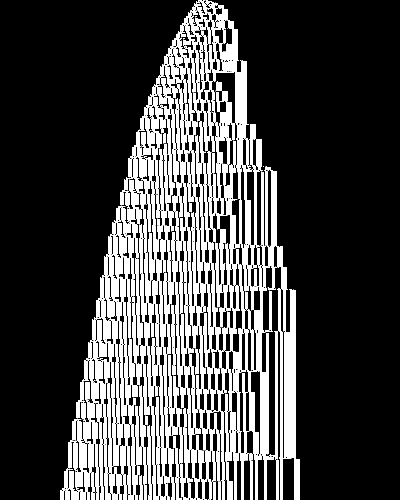
\includegraphics[scale=0.35]{figures/bouncers/5608043.png}
    \caption{\small 50,000-step space-time diagram of \url{https://bbchallenge.org/5608043}. Out of the 29,799 decided bouncers, this bouncer takes the most steps (141,509) to be detected and fits the biggest formula tape, using Algorithm~\ref{alg:decider-bouncers} presented in this section.}\label{fig:big-bounce}
\end{figure}
\vspace{-2.5ex}
\paragraph*{Remarkable bouncers.} Out of the 29,799 bouncers that were decided using Algorithm~\ref{alg:decider-bouncers}, here are some remarkable facts:
\begin{enumerate}
    \item Using Algorithm~\ref{alg:decider-bouncers}, only two bouncers with 3 repeaters were found (and that's the maximum): \url{https://bbchallenge.org/347505} and \url{https://bbchallenge.org/8131743}. Otherwise, 2132 bouncers have 2 repeaters and the rest has only 1.
    \item\label{pt:big-formula-tape} The biggest fitted formula tapes by the algorithm have 328 symbols (summing walls and repeater symbols, not counting head and $0^\infty$), there are two of them, such as for machine \url{https://bbchallenge.org/5608043}, see Figure~\ref{fig:big-bounce}:
          \begin{align*}
               & 0^\infty\lhead{\text{A}}  10000011100011100000011100001110111001110111001110000111 \\ &0000111011100111000011101110011101110011100001110000111011100\\ &1110000111000011100001110000111011100111011100111011100111011\\ &100111011100111011100(111011100111011100111011100111011100)000\\ &1110000111000000111001111111111111110000111(111111111111)00111\\ &000000011100000011111100111111(0)^\infty
          \end{align*}

    \item The above machine of Point~\ref{pt:big-formula-tape} is also the machine that is detected after the most steps: 141,509. Over this dataset, it took 207 steps on average.
    \item The most macro steps (i.e.\ number of usual or shift rule steps in formula tape simulation) needed to conclude using Theorem~\ref{th:bouncers} was 41,628 for \url{https://bbchallenge.org/347505}. Otherwise, it took 66 macro steps on average.

\end{enumerate}
